\documentclass[12pt]{beamer}
\usetheme{CambridgeUS}
\usepackage[utf8]{inputenc}
\usepackage[spanish]{babel}
\usepackage{amsmath}
\usepackage{amsfonts}
\usepackage{amssymb}
\usepackage{graphicx}
\author{Kevin Garcia - Cesar Saavedra}
\title{Taller: Modelos de distribución}
%\setbeamercovered{transparent} 
%\setbeamertemplate{navigation symbols}{} 
%\logo{} 
%\institute{} 
%\date{} 
%\subject{} 
\begin{document}

\begin{frame}
\titlepage
\end{frame}

%\begin{frame}
%\tableofcontents
%\end{frame}
\begin{frame}
\frametitle{Distribución Poisson}
~\\  Esta distribución es una de las más importantes distribuciones de variable discreta. Sus principales aplicaciones hacen referencia a la modelización de situaciones en las que nos interesa determinar el número de hechos de cierto tipo que se pueden producir en un intervalo de tiempo o de espacio, bajo presupuestos de aleatoriedad.
~\\ Su función de densidad esta dada por: 
~\\$$f(x,\lambda)=\frac{e^{-\lambda}\cdot \lambda^x}{x!}  ; x \in \{0,1,2,3,...\}$$
~\\donde:
\begin{itemize} 
\item x es el número de ocurrencias del evento o fenómeno (la función nos da la probabilidad de que el evento suceda precisamente x veces).
\end{itemize}
\end{frame}

\begin{frame}
\frametitle{Distribución Poisson}
\begin{itemize}
\item $\lambda$ es un parámetro positivo que representa el número de veces que se espera que ocurra el fenómeno durante un intervalo dado.
\item $F(x)=\sum\limits_{i=1}^{x} \frac{\lambda_{i}\cdot e^{-\lambda}}{i!}$
\item $f.g.m=m_{x}(t)=E[e^{tx}]=\sum\limits_{x} e^{tx}p(x)= e^{[\lambda(e^t-1)]}$
\item $Media=E[x]=\lambda$
\item $Varianza=\lambda$
\item Coeficiente de asimetría=$\frac{1}{\sqrt{\lambda}}$
\item curtosis=$3+\frac{1}{\lambda}$
\end{itemize}
\end{frame}

\begin{frame}
\frametitle{Aplicaciones de la distribución Poisson}
~\\La distribución de Poisson se emplea para describir procesos como los siguientes:  
\begin{itemize}
\item El número de autos que pasan a través de un cierto punto en una ruta (suficientemente
distantes de los semáforos) durante un periodo definido de tiempo.  
\item El número de errores de ortografía que uno comete al escribir una única página.  
\item El número de llamadas telefónicas en una central telefónica por minuto.  
\item El número de servidores web accedidos por minuto.  
\item El número de defectos en una longitud específica de una cinta magnética.   
\item El número de defectos por metro cuadrado de tela.
\item El número de estrellas en un determinado volumen de espacio.
\end{itemize}
\end{frame}
\begin{frame}
\frametitle{Distribución Logística}
~\\La función de distribución de la logística es una distribución de probabilidad continua que se usa como modelo de crecimiento. Por ejemplo,
con un nuevo producto, a menudo encontramos que el crecimiento es inicialmente lento, luego gana impulso,
y finalmente se ralentiza cuando el mercado está saturado o hay alguna forma de equilibrio
alcanzado
~\\ Su función de densidad está dada por:
$$f(x;a,b)=\frac{e^{-(x-a)/b}}{b(1+e^{-(x-a)/b})^2}=\frac{1}{4b}sech^2\left(\frac{x-a}{2b}\right)$$
\end{frame}

\begin{frame}
\frametitle{Distribución Logística}
~\\ Su función de distribución está dada por:
$$F(x;a,b)=\frac{1}{1+e^{-(x-a)/b}}=\frac{1}{2}+\frac{1}{2}tanh\left(\frac{x-a}{2b}\right)$$
\begin{itemize}
\item $f.g.m=e^{at}\Gamma(1-bt)\Gamma(1+bt)=\pi bt\frac{e^{at}}{sin(\pi bt)}$
\item $Media=E[x]=a$
\item $Mediana=a$
\item $Moda=a$
\item $Varianza=\frac{\pi^2 b^2}{3}$
\end{itemize}
\end{frame}

\begin{frame}
\frametitle{Aplicaciones de la distribución Logística}
~\\ La distribución logística ha sido muy utilizada en áreas como:
\begin{itemize}
\item Biología: para describir cómo se comportan las especies en entornos competitivos.
\item Epidemiología: para describir la propagación de epidemias.
\item Psicología: para describir el proceso de aprendizaje.
\item Tecnología: para describir cómo las tecnologías se popularizan y compiten entre sí.
\item Márketing: para estudiar la difusión de nuevos productos.
\item Energía: para estudiar la difusión y sustitución de unas fuentes de energía primarias por otras.
\end{itemize}
\end{frame}

\begin{frame}
\frametitle{Comportamiento distribución Poisson}

\end{frame}
\begin{frame}
\frametitle{Comportamiento distribución Logística}

\end{frame}

\begin{frame}
\frametitle{Variable 'Edad mediana de las viviendas'}
\begin{figure}[!h]
    \begin{center}
        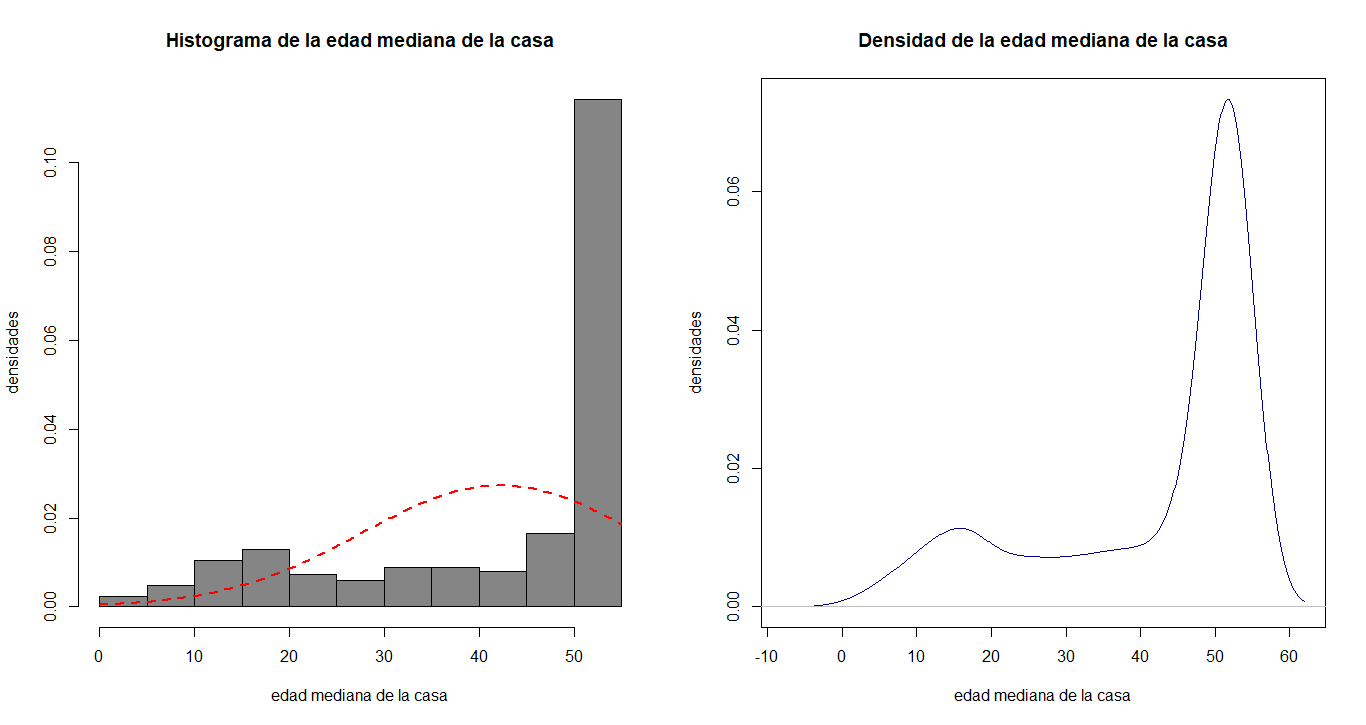
\includegraphics[width=11cm]{imagenes/3.png}
        \caption{Histograma y densidad de la variable 'Edad mediana de las viviendas'}
        \label{fig:Densidad}
    \end{center}
\end{figure}
\end{frame}
\begin{frame}
\frametitle{Variable 'Edad mediana de las viviendas'}
\begin{figure}[!h]
    \begin{center}
        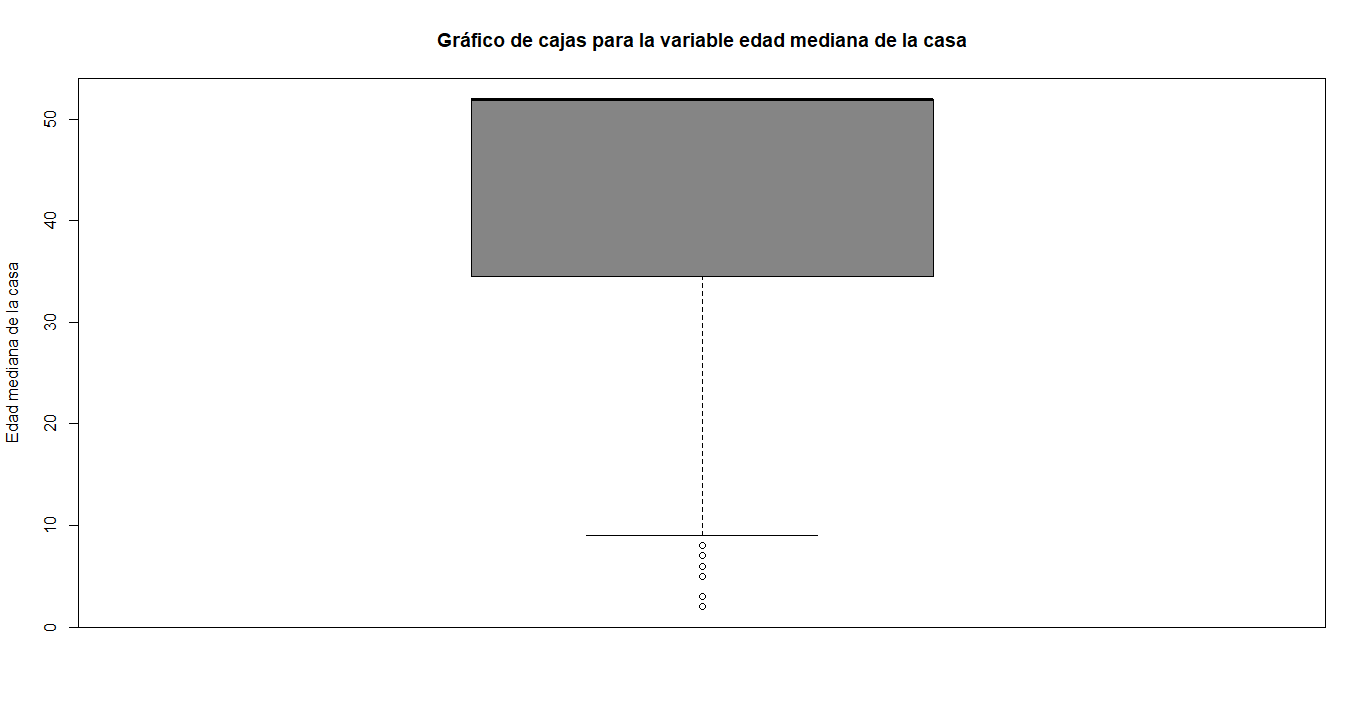
\includegraphics[width=11cm]{imagenes/14.png}
        \caption{Gráfico de cajas para la variable 'Edad mediana de las viviendas'}
        \label{fig:Densidad}
    \end{center}
\end{figure}
\end{frame}

\begin{frame}
\frametitle{Variable 'Total de habitaciones'}
\begin{figure}[!h]
    \begin{center}
        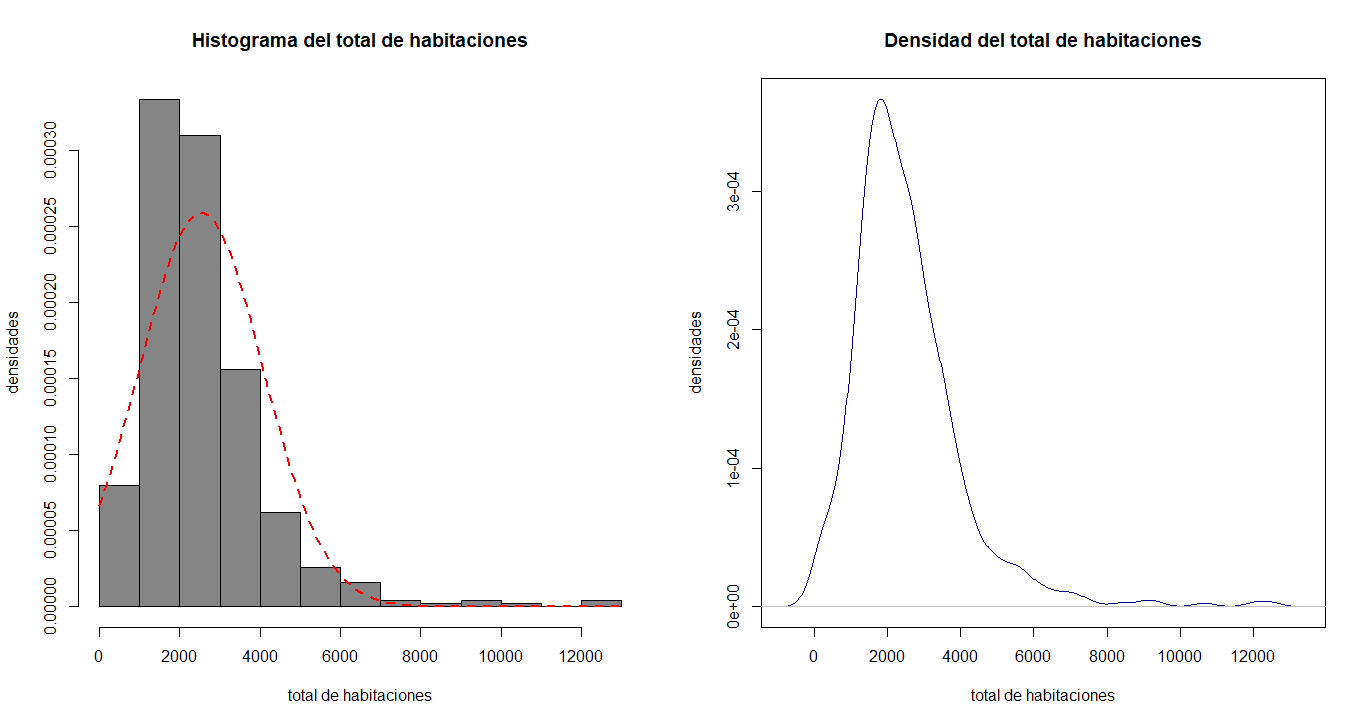
\includegraphics[width=11cm]{imagenes/4.png}
        \caption{Histograma y densidad de la variable 'Total de habitaciones'}
        \label{fig:Densidad}
    \end{center}
\end{figure}
\end{frame}
\begin{frame}
\frametitle{Variable 'Total de habitaciones'}
\begin{figure}[!h]
    \begin{center}
        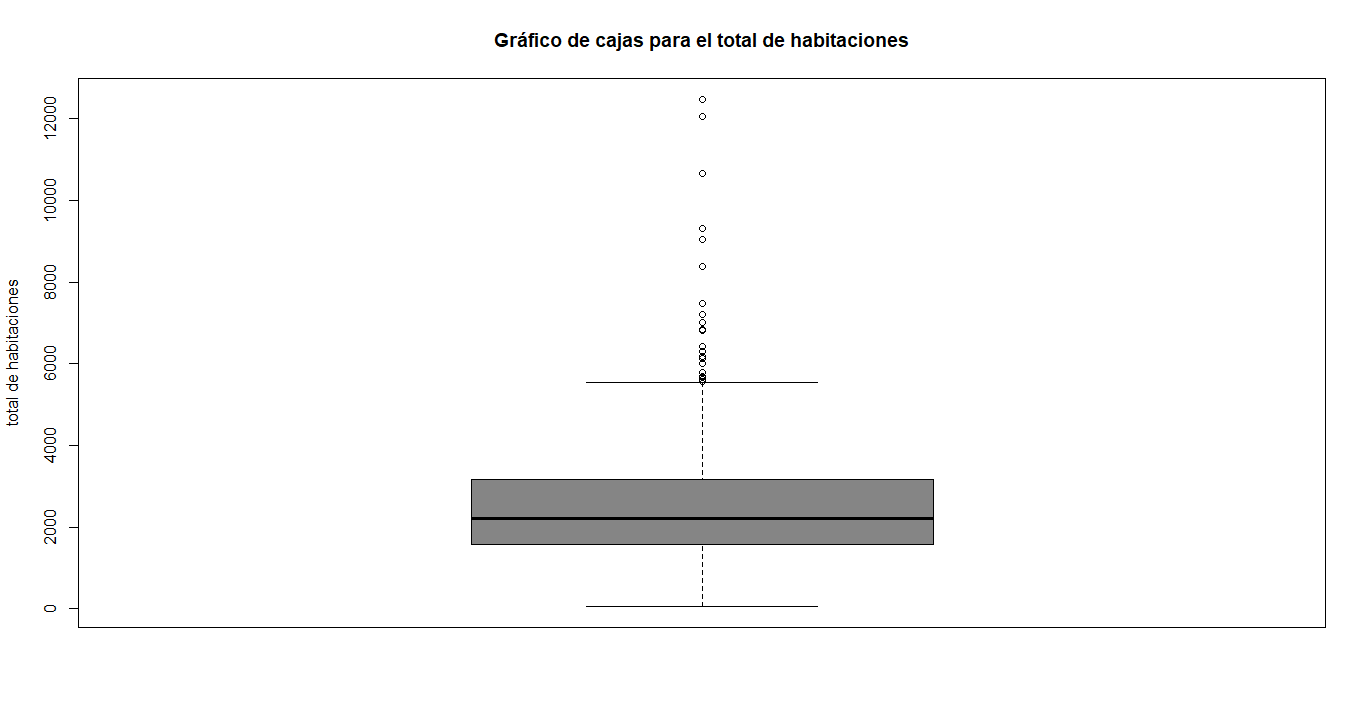
\includegraphics[width=11cm]{imagenes/15.png}
        \caption{Gráfico de cajas para la variable 'Total de habitaciones'}
        \label{fig:Densidad}
    \end{center}
\end{figure}
\end{frame}

\begin{frame}
\frametitle{Variable 'Total de dormitorios'}
\begin{figure}[!h]
    \begin{center}
        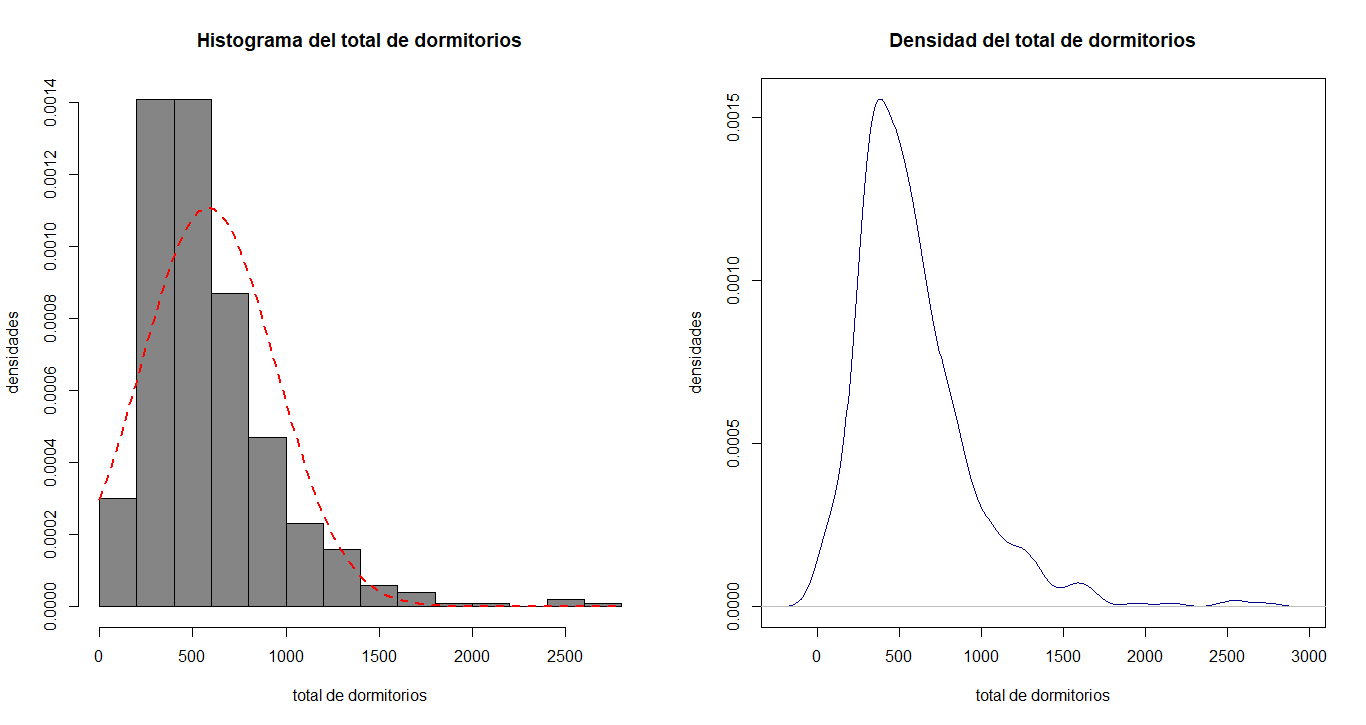
\includegraphics[width=11cm]{imagenes/5.png}
        \caption{Histograma y densidad de la variable 'Total de dormitorios'}
        \label{fig:Densidad}
    \end{center}
\end{figure}
\end{frame}
\begin{frame}
\frametitle{Variable 'Total de dormitorios'}
\begin{figure}[!h]
    \begin{center}
        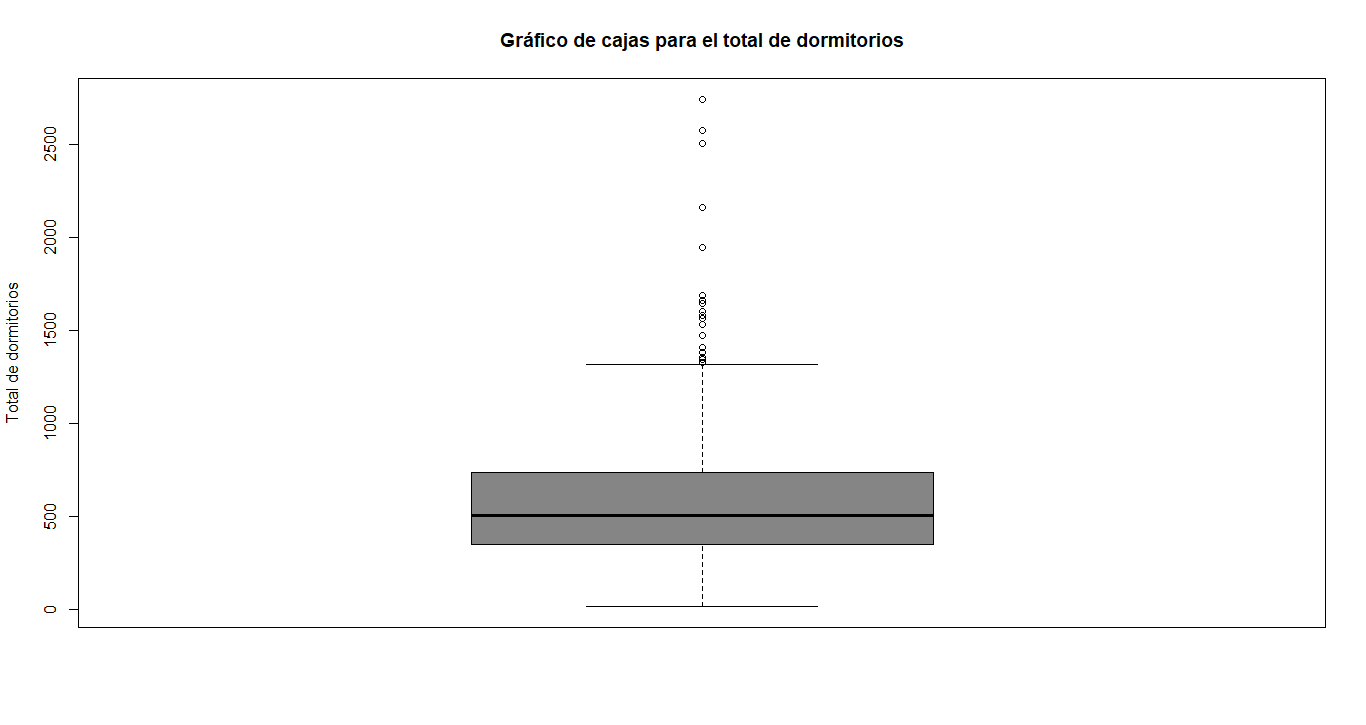
\includegraphics[width=11cm]{imagenes/16.png}
        \caption{Gráfico de cajas para la variable 'Total de dormitorios'}
        \label{fig:Densidad}
    \end{center}
\end{figure}
\end{frame}
\begin{frame}
\frametitle{Variable 'Población'}
\begin{figure}[!h]
    \begin{center}
        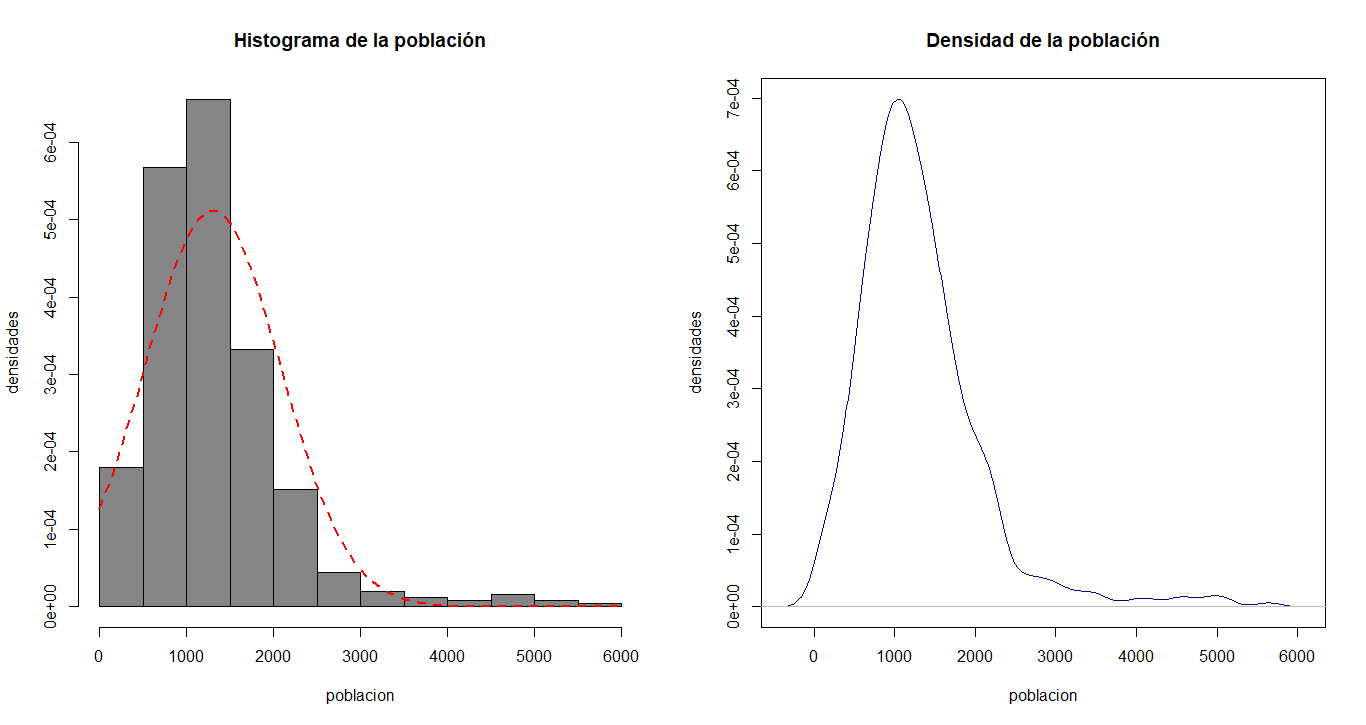
\includegraphics[width=11cm]{imagenes/6.png}
        \caption{Histograma y densidad de la variable 'Población'}
        \label{fig:Densidad}
    \end{center}
\end{figure}
\end{frame}
\begin{frame}
\frametitle{Variable 'Población'}
\begin{figure}[!h]
    \begin{center}
        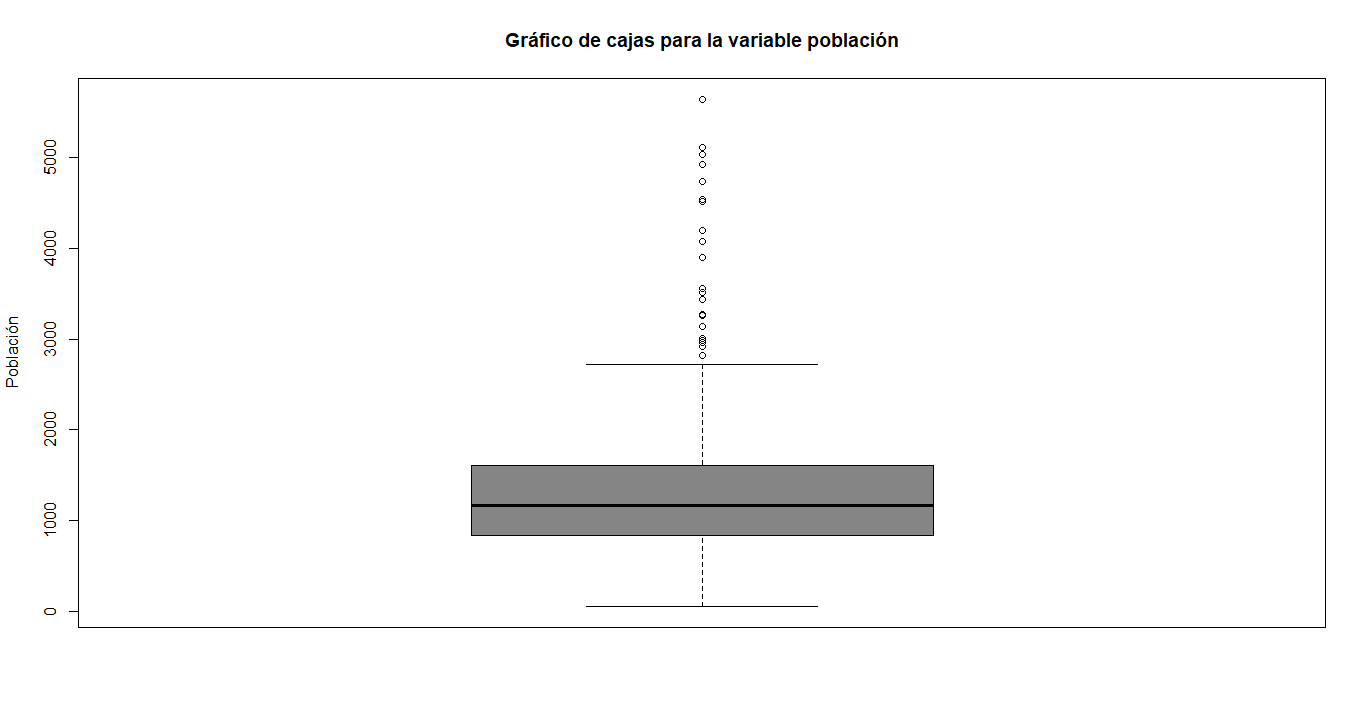
\includegraphics[width=11cm]{imagenes/17.png}
        \caption{Gráfico de cajas para la variable 'Población'}
        \label{fig:Densidad}
    \end{center}
\end{figure}
\end{frame}

\begin{frame}
\frametitle{Variable 'Hogares'}
\begin{figure}[!h]
    \begin{center}
        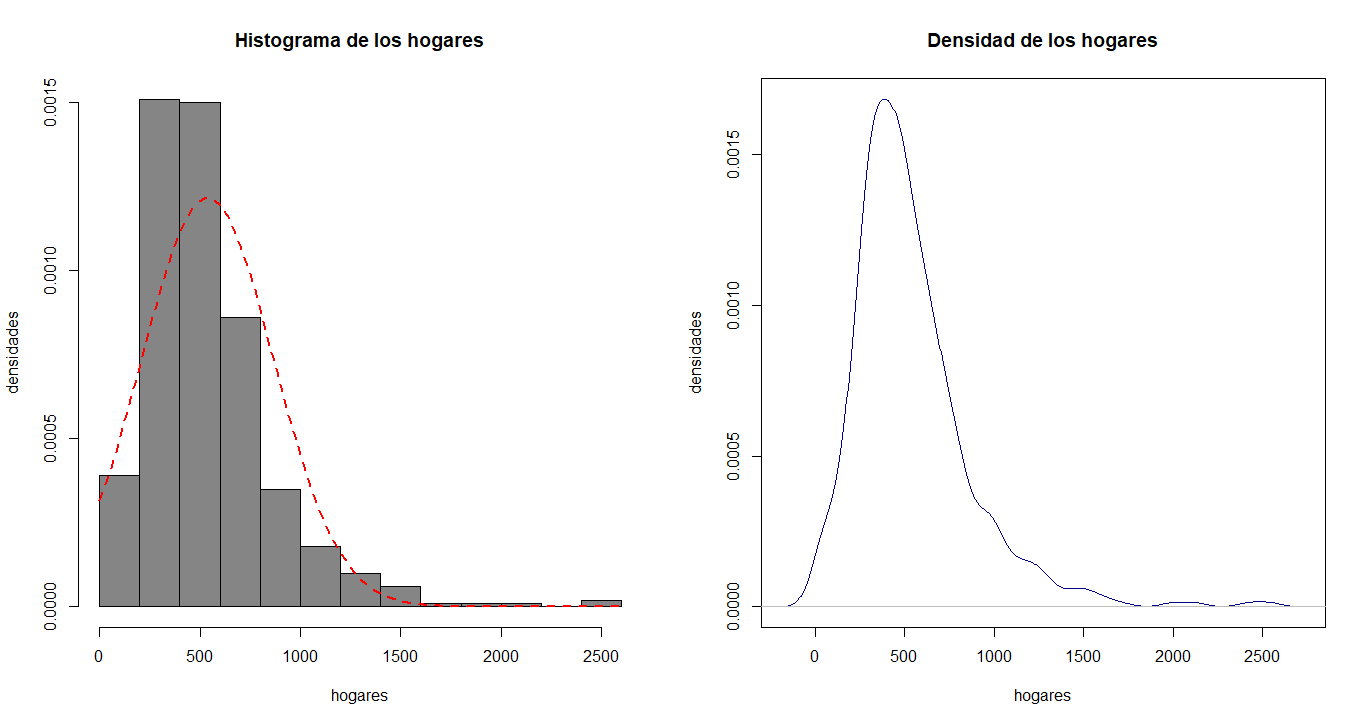
\includegraphics[width=11cm]{imagenes/7.png}
        \caption{Histograma y densidad de la variable 'Hogares'}
        \label{fig:Densidad}
    \end{center}
\end{figure}
\end{frame}
\begin{frame}
\frametitle{Variable 'Hogares'}
\begin{figure}[!h]
    \begin{center}
        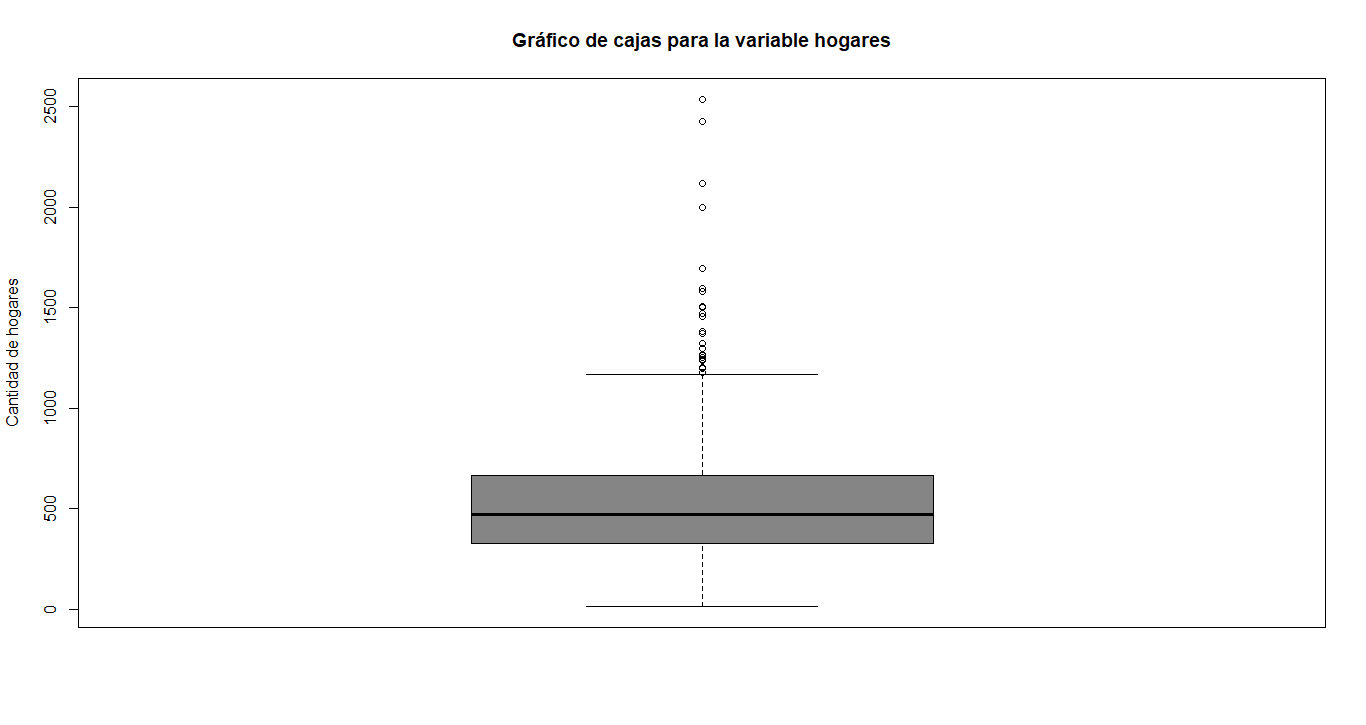
\includegraphics[width=11cm]{imagenes/18.png}
        \caption{Gráfico de cajas para la variable 'Hogares'}
        \label{fig:Densidad}
    \end{center}
\end{figure}
\end{frame}

\begin{frame}
\frametitle{California}
\begin{figure}[!h]
    \begin{center}
        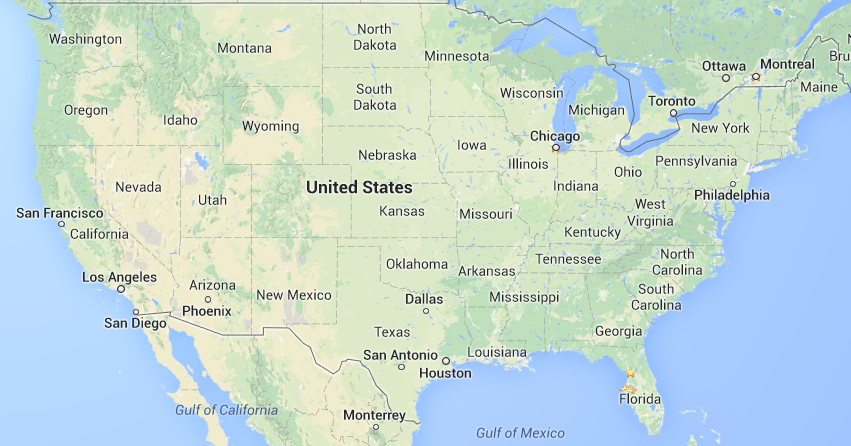
\includegraphics[width=11cm]{imagenes/california.png}
        \caption{Lugar de donde provienen los datos}
        \label{fig:Densidad}
    \end{center}
\end{figure}
\end{frame}

\begin{frame}
\frametitle{San Francisco}
\begin{figure}[!h]
    \begin{center}
        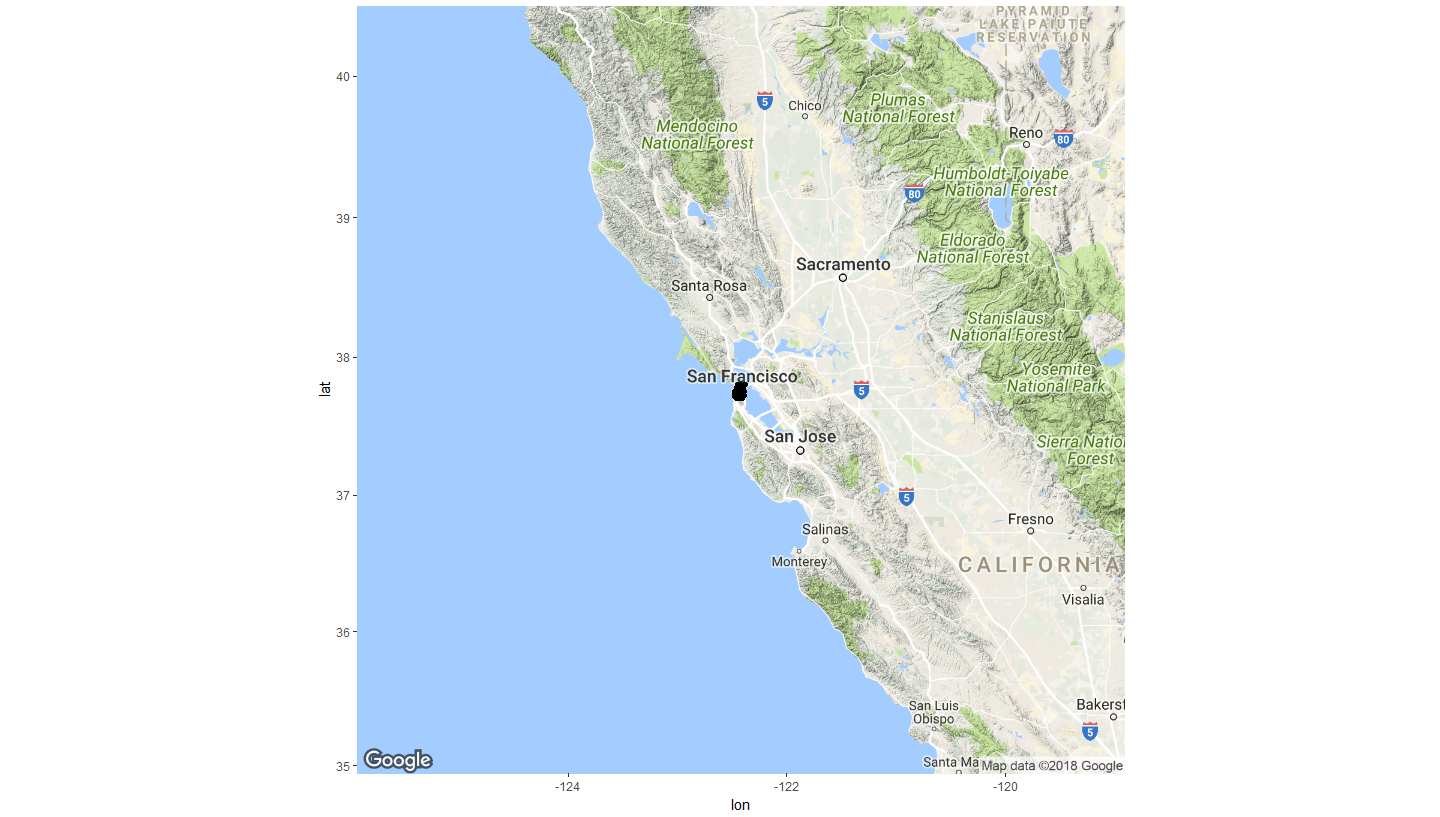
\includegraphics[width=11cm]{imagenes/sanfransisco.png}
        \caption{Mapa con los puntos dados de longitud y latitud}
        \label{fig:Densidad}
    \end{center}
\end{figure}
\end{frame}

\begin{frame}
\frametitle{San Diego}
\begin{figure}[!h]
    \begin{center}
        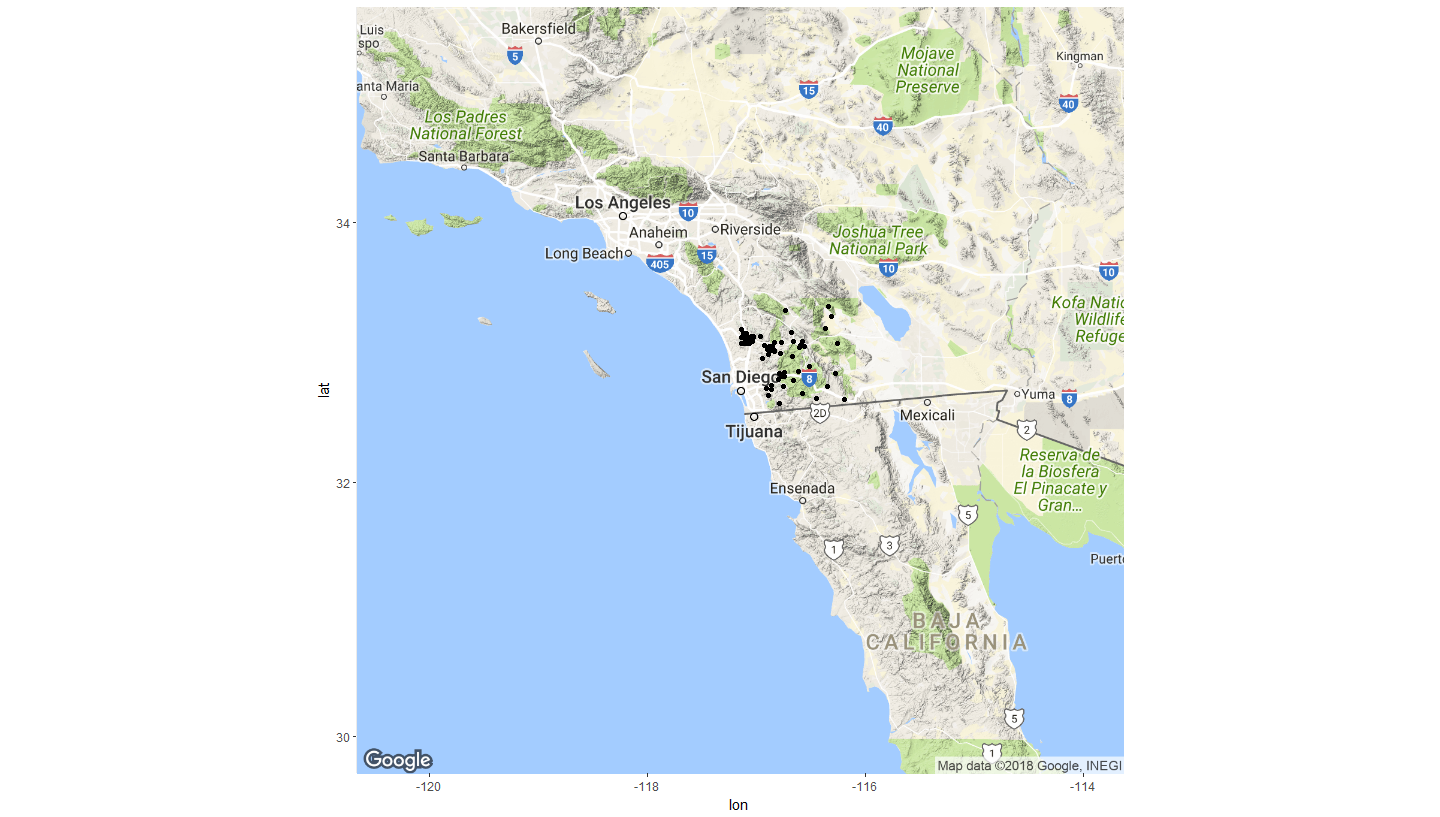
\includegraphics[width=11cm]{imagenes/sandiego.png}
        \caption{Mapa con los puntos dados de longitud y latitud}
        \label{fig:Densidad}
    \end{center}
\end{figure}
\end{frame}

\begin{frame}
\frametitle{Posibles relaciones entre las variables explicativas}
\begin{itemize}
\item Matriz de correlaciones:
\begin{figure}[!h]
       \raggedright
        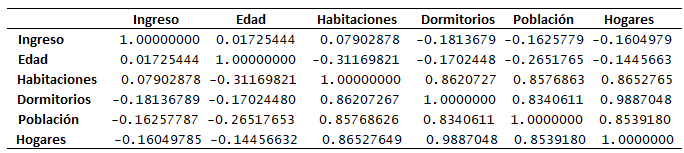
\includegraphics[width=11.2cm]{imagenes/correlacion.png}
        \caption{Matriz de correlaciones entre covariables }
        \label{fig:Densidad}
\end{figure}
\end{itemize}
\end{frame}

\begin{frame}
\frametitle{Posibles relaciones entre las variables explicativas}
\begin{itemize}
\item Variables 'Total de dormitorios' y 'Hogares':
\begin{figure}[!h]
    \begin{center}
        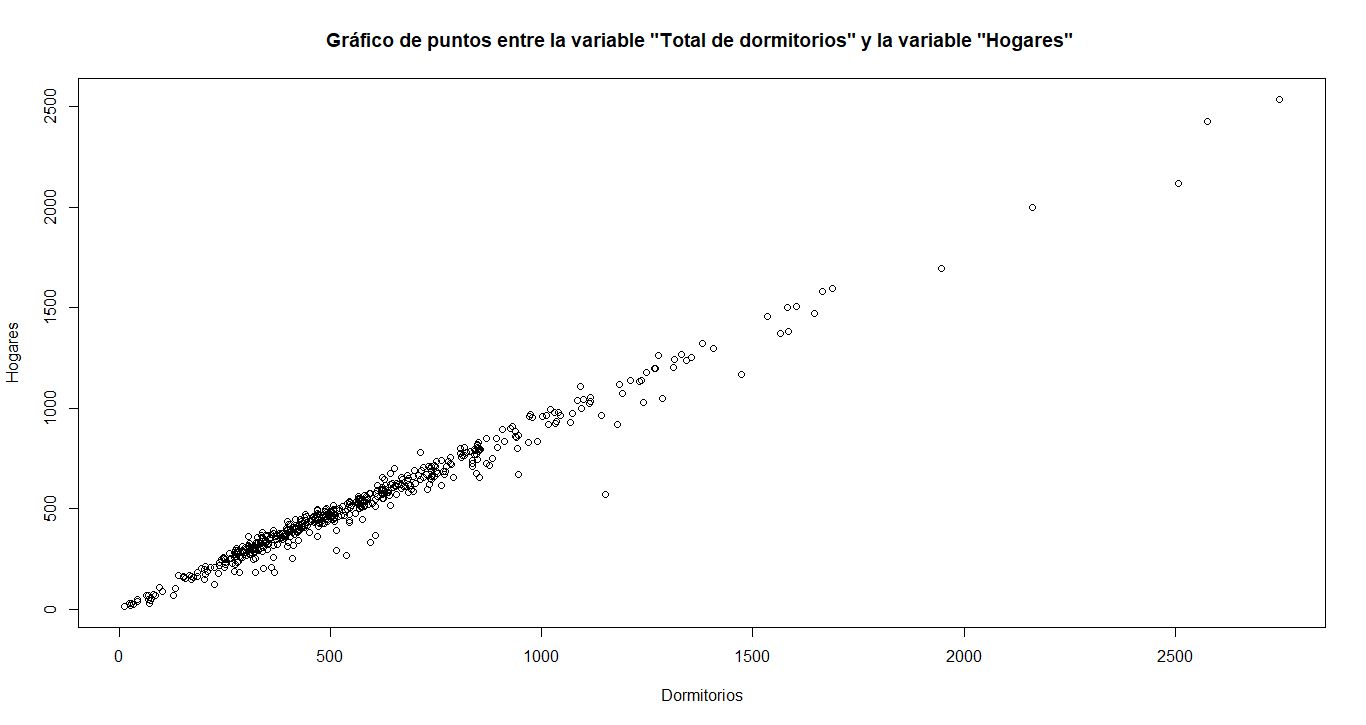
\includegraphics[width=10cm]{imagenes/19.png}
        \caption{Gráfico de puntos entre las variables 'Total de dormitorios' y 'Hogares'}
        \label{fig:Densidad}
    \end{center}
\end{figure}
\end{itemize}
\end{frame}

\begin{frame}
\frametitle{Posibles relaciones entre las variables explicativas}
\begin{itemize}
\item correlación de Pearson: $r=0.9887048$
\item correlación de Spearman: $\rho=0.9819133$
\end{itemize}
\end{frame}

\begin{frame}
\frametitle{Posibles relaciones entre las variables explicativas}
\begin{itemize}
\item Variables 'Población' y 'Hogares':
\begin{figure}[!h]
    \begin{center}
        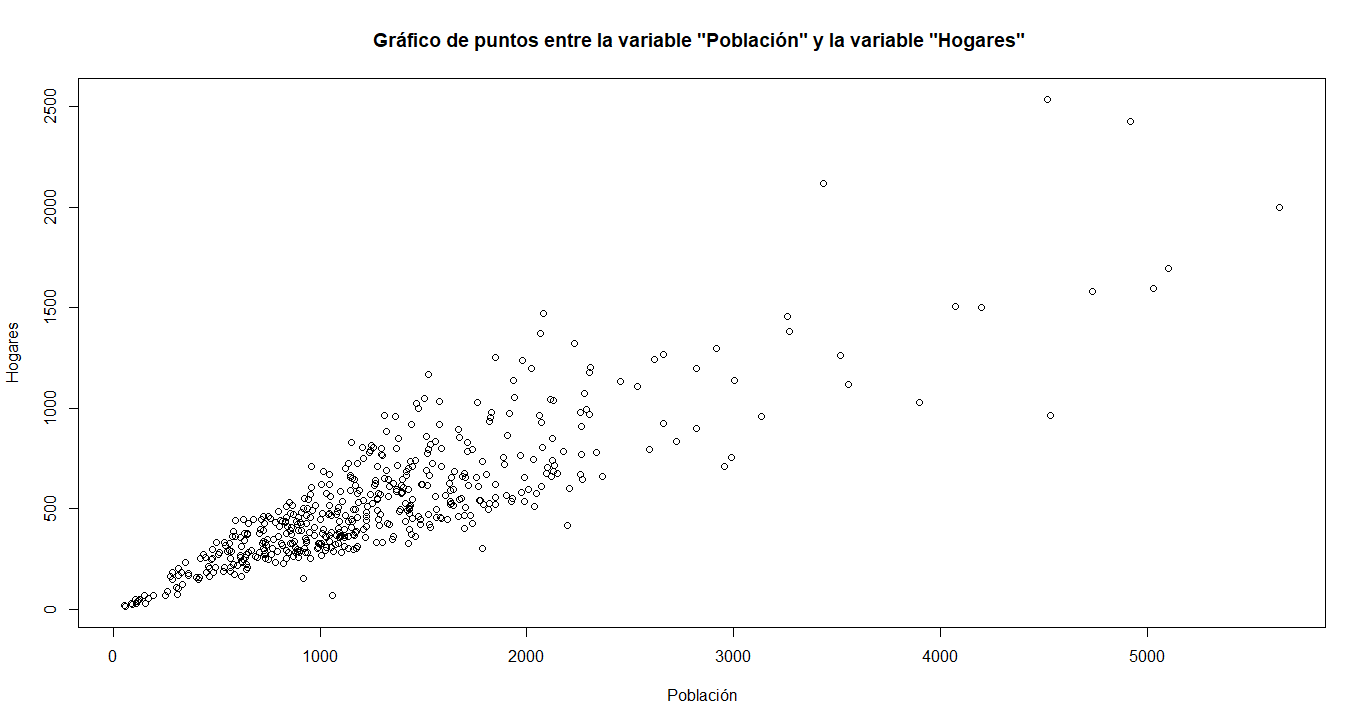
\includegraphics[width=10cm]{imagenes/10.png}
        \caption{Gráfico de puntos entre las variables 'Población' y 'Hogares'}
        \label{fig:Densidad}
    \end{center}
\end{figure}
\end{itemize}
\end{frame}

\begin{frame}
\frametitle{Posibles relaciones entre las variables explicativas}
\begin{itemize}
\item correlación de Pearson: $r=0.853918$
\item correlación de Spearman: $\rho=0.8395669$
\end{itemize}
\end{frame}

\begin{frame}
\frametitle{Posibles relaciones entre las variables explicativas}
\begin{itemize}
\item Variables 'total de habitaciones' y 'total de dormitorios':
\begin{figure}[!h]
    \begin{center}
        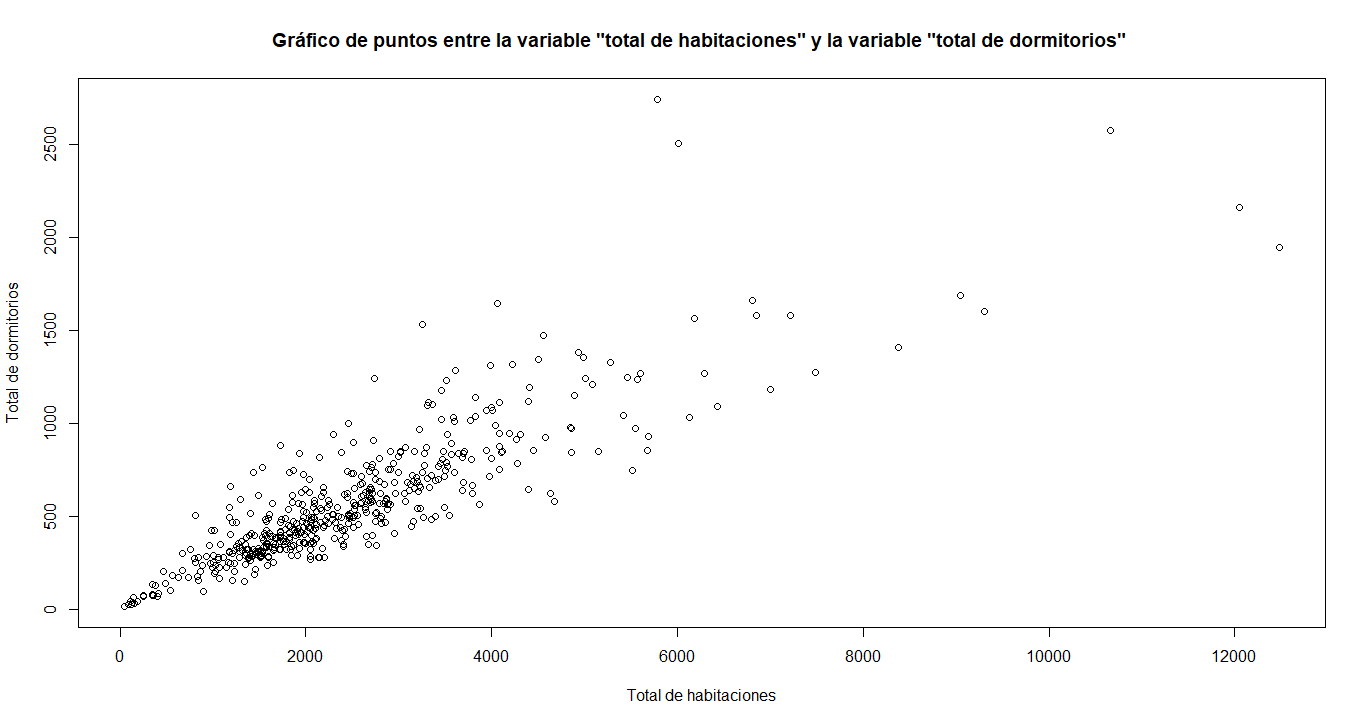
\includegraphics[width=10cm]{imagenes/11.png}
        \caption{Gráfico de puntos entre las variables 'total de habitaciones' y 'total de dormitorios'}
        \label{fig:Densidad}
    \end{center}
\end{figure}
\end{itemize}
\end{frame}

\begin{frame}
\frametitle{Posibles relaciones entre las variables explicativas}
\begin{itemize}
\item correlación de Pearson: $r=0.862072$
\item correlación de Spearman: $\rho=0.8716658$
\end{itemize}
\end{frame}

\begin{frame}
\frametitle{Modelo ajustado e interpretación}
~\\ El modelo ajustado incluyendo todas las variables sin transformación y sin selección de variables es:
~\\ $Y=57720.52+24261.20X_{1}+3443.94X_{2}+19.09X_{3}-67.72X_{4}-121.66X_{5}+315.92X_{6}$

~\\ Donde: Y=Valor mediano de la casa, $X_{1}=$Ingreso mediano, $X_{2}=$Edad mediana de la vivienda, $X_{3}=$Total de habitaciones, $X_{4}=$Total de dormitorios, $X_{5}=$Población, $X_{6}=$Hogares.
\begin{itemize}
\item $R^2=0.5425$
\item $R^2_{ajustado}=0.537$
\item $CME=\hat{\sigma^2}=6724487923$
\end{itemize}
\end{frame}


\begin{frame}
\frametitle{Modelo ajustado e interpretación}
\begin{itemize}
\item $\beta_{0}$:Representa el valor del intercepto con el eje y, esto quiere decir que Y va a partir de un valor de 57720.52 sin importar en cuantas unidades aumente mis otras variables.  
\item $\beta_{1}$:por cada unidad que aumente de ingreso mediano se aumentan 24261.20 unidades del valor mediano de la casa.
\item $\beta_{2}$:por cada unidad que aumente de edad mediana de la vivienda se aumentan 3443.94 unidades del valor mediano de la casa.
\item $\beta_{3}$:por cada unidad que aumente de total de habitaciones se aumentan 19.09 unidades del valor mediano de la casa.
\item $\beta_{4}$:por cada unidad que aumente de total de dormitorios se disminuye 67.72 unidades del valor mediano de la casa.
\end{itemize}
\end{frame}
\begin{frame}
\begin{itemize}
\item $\beta_{5}$:por cada unidad que aumente de población se disminuye 121.66 unidades del valor mediano de la casa.
\item $\beta_{6}$:por cada unidad que aumente de hogares se aumenta 315.92 unidades del valor mediano de la casa.
\end{itemize}
\end{frame}

\begin{frame}
\frametitle{Modelo ajustado con selección de variables}
~\\ El modelo ajustado, utilizando el método forward para seleccionar variables es exactamente el mismo modelo completo, es decir, el método no me elimino ninguna variable.
\end{frame}

\begin{frame}
\frametitle{Modelo ajustado con selección de variables}
~\\ El modelo ajustado, utilizando el método backward para seleccionar variables es:
~\\ $Y=52921.688+24923.244X_{1}+3484.164X_{2}+17.588X_{3}-118.652X_{5}+243.265X_{6}$

~\\ Donde: Y=Valor mediano de la casa, $X_{1}=$Ingreso mediano, $X_{2}=$Edad mediana de la vivienda, $X_{3}=$Total de habitaciones, $X_{5}=$Población, $X_{6}=$Hogares.
\begin{itemize}
\item $R^2=0.5417$
\item $R^2_{ajustado}=0.5371$
\item $CME=\hat{\sigma^2}=6722361839$
\end{itemize}
\end{frame}

\begin{frame}
\frametitle{Modelo ajustado con selección de variables}
~\\ El modelo ajustado, utilizando el método stepwise para seleccionar variables es  exactamente el mismo modelo que ajustamos por el método anterior (backward), es decir, ambos métodos nos eliminan la variable $X_{4}=$Total de dormitorios del modelo completo.
\end{frame}

\begin{frame}
\frametitle{Comparación}
\begin{figure}[!h]
    \begin{center}
        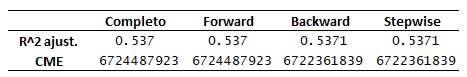
\includegraphics[width=11cm]{imagenes/comparacion.png}
        \caption{Comparación de los modelos generados con selección de variables}
        \label{fig:Densidad}
    \end{center}
\end{figure}
\end{frame}

\begin{frame}
\frametitle{Conclusión}
~\\ Al finalizar nuestra selección de variables, con el fin de ajustar el mejor modelo posible para la variable valor mediano de la casa, comparamos cada uno de los 4 modelos obtenidos (completo, forward, backward, stepwise) con respecto al $R^2_{ajustado}$ y el $CME=\hat{\sigma^2}$. Podemos concluir que el mejor modelo que logramos obtener  para nuestros 500 datos sin hacer transformación de variables, fue el generado por el método de selección 'Backward'      y 'Stepwise', los cuales nos eliminaron la variable explicativa $X_{4}:$Total de dormitorios.
\end{frame}

\end{document}